We have implemented our approach in a prototype and compared it 3 types of related approaches (i) \deeppoly{}~\cite{singh2019abstract} and its refinements \texttt{kPoly}~\cite{singh2019beyond}, \texttt{deepSRGR}~\cite{yang2021improving}, (ii) other cegar based approaches and 
%The approaches  \texttt{kPoly} and \texttt{deepSRGR} do the refinement on \deeppoly{}.
(iii) state-of-the-art tools \alphabeta~\cite{alphabetacrown} and \ovaltool~\cite{ovaltool}, both of which use a set/portfolio of different algorithms and optimizations. The first tool~\alphabeta achieved the 1st and \ovaltool 3rd rank in the 2nd International Verification of Neural Networks Competition (VNN-COMP'21).
%We use the MNIST \cite{deng2012mnist} for our evaluation.    
\subsection{Implementation}
We have implemented our techniques in a tool, which we call \drefine{}, in \texttt{C++} programming language. Our approach relies on \deeppoly{}, so we also have implemented \deeppoly{} in \texttt{C++}. We are using a \texttt{C++} interface of the tool Gurobi~\cite{?} \todo{add ref} to check the satisfiability as well as solve  \texttt{maxsat} queries. %We have implemented our technique as a tool and call it \drefine{}.  

\subsection{Benchmarks}
We use the MNIST~\cite{deng2012mnist} dataset to check the effectiveness of our tool and comparisons. We are using 11 different fully connected feedforward neural networks with $\relu${} activation as shown in table~\ref{tb:nndetail}.
These benchmarks are taken from the \deeppoly{}'s paper~\cite{singh2019abstract}.  The input and output dimensions of each network are $784$ and $10$ respectively. 
The authors of \deeppoly{} used projected gradient descent (PGD)~\cite{dong2018boosting}
and DiffAI~\cite{mirman2018differentiable} for adversarial training. Table \ref{tb:nndetail} contains the defended network i.e.
trained with adversarial training as well as the undefended network. The last column of the table \ref{tb:nndetail} how the defended networks were trained.  

The predicate $P$ on the input layer is created using the input image $\boldsymbol{im}$ and user-defined parameter $\epsilon$.  We first normalize each pixel of $\boldsymbol{im}$ between $0$ and $1$, then create  $P = \Land_{i=1}^{|l_0|} im(i)-\epsilon \leq x_{0i}\leq im(i)+\epsilon$, such that the lower and upper bound of each pixel should not exceed $0$ and $1$ respectively. The predicate $Q$ on the output layer is created using the network's output.     Suppose the predicted label of $\boldsymbol{im}$ on network $N$ is $y$, then $Q = \Land_{i=1}^{|l_k|} x_{ki} < y$, where $i \neq y$.  One query instance $\langle N,P,Q \rangle$ is created for one network, one image and one epsilon value.  In our evaluation, we took $11$ different networks, 8 different epsilons, and 100 different images. The 
total number of instances is computed to $8800$. However, there are 128 instances for which the network's predicted label differs from the image's actual label. we avoided such instances, so, there is a total of $8672$ benchmark instances
under consideration.    Whenever our tool found a counter-example on $\langle N,P,Q \rangle$, it denormalizes it into an image by rounding the float values 
and checks for counter-example by executing $N$ on the denormalized image.
If a counter-example is found then the tool reports it, otherwise, the tool reports unknown.



\begin{table}[t]
    \centering
    \begin{tabular}{c|c|c|c}
        \hline
        \textbf{Neural Network} & \textbf{\#hidden layers} & \textbf{\#activation units} & \textbf{Defensive training} \\
        \hline
        $3\times 50$ & 2 & 110 & None \\
        $3\times 100$ & 2 & 210 & None  \\
        $5\times 100$ & 4 & 410 & None  \\
        $6\times 100$ & 5 & 510 & DiffAI \\
        $9\times 100$ & 8 & 810 & None  \\
        $6\times 200$ & 5 & 1010 & None  \\
        $9\times 200$ & 8 & 1610 & None  \\
        $6\times 500$ & 6 & 3000 & None  \\
        $6\times 500$ & 6 & 3000 & PGD, $\epsilon = 0.1$ \\
        $6\times 500$ & 6 & 3000 & PGD, $\epsilon = 0.3$ \\
        $4\times 1024$ & 3 & 3072 & None  \\
        \hline
    \end{tabular}
    \caption{Neural networks details}
    \label{tb:nndetail}
\end{table}

\subsection{Results}
We conducted the experiments on a machine with \texttt{64GB RAM, 2.20 GHz Intel(R) Xeon(R) CPU E5-2660 v2}
processor with CentOS Linux 7 operating system. 
To make a fair comparison between the tools, we provide only a single \texttt{CPU} for each benchmarks instances for each tool. 
We make three types of comparisons as shown in (i) Figure~\ref{res:milp_with_milp}, which is a cactus plot of (log of) time taken vs the number of benchmarks solved (ii) Table~\ref{tb:matrix}, which makes a pairwise comparison of the number of instances that a tool could solve which another couldn't  (more precisely, the $(i,j)$-entry of the table is the number of instances which could be verified by tool $i$ but not by tool $j$) and (iii) Figure~\ref{res:ep:milp_with_milp} which compares wrt epsilon, the robustness parameter.
%represents the verified cases while the column represents the not verified cases, i.e.\kpoly{}'th row and \deeppoly{}'th column represent the  156 number of benchmarks instances which are solved by \kpoly{} and not solved by \deeppoly{}. 

We remark that on an average, \drefine{} marks $9.8\%$ of neurons, whenever it needs to refine.  \todo{probably should be moved somewhere else?}

\subsubsection{Comparison with the most related techniques:}
In this subsection, we consider the techniques \deeppoly{}, \kpoly{}, and \deepsrgr{} to compare with our technique. 
We consider \deeppoly{} because it is at the base of our technique, and the techniques \kpoly{} and \deepsrgr{} refine \deeppoly{} just as we do. These tools only report \texttt{verified} instances, while our tool can report  \texttt{verified} and the counter-example. We note that we compare these techniques with only \texttt{verified}  instances of our technique in the line of \texttt{drefine\_verified} in cactus plot ~\ref{res:milp_with_milp}. 

It can be seen that our technique outperforms the others in terms of the verified number of instances. One can also see that when they do verify, \deeppoly{} and \kpoly{} are efficient compared to our tool which is not surprising, while our tool is more efficient than \deepsrgr{}. From Table~\ref{tb:matrix}, we also see  that our tool solves all the benchmark instances which are solved by these three techniques (and significantly more ~3700 for the first two and ~1000 for the third), except $14$ instances where \kpoly{} succeeds and our tool times out.

% The approaches \deeppoly{}, \texttt{refinepoly}, and \texttt{deepSRGR} are incomplete and do not report the counter-example. 
% Our approach is a complete approach. We compare our approach's \texttt{verified} only instances with incomplete approaches. 
% Figure~\ref{res:milp_with_milp} shows the comparison with the help of the cactus plot. Our approach performs well 
% in terms of the verified number of instances as well as in terms of time in comparison to the above incomplete approaches. 
% We are also comparing with state of the arts to check the effectiveness of our approach globally.
% Table~\ref{tb:soacomparison} shows that our tool is verifying $180$ and $190$ benchmarks which $\alpha -\beta$-CROWN and 
% \texttt{oval} respectively are not able to verify. In addition to this, our tool verifies $172$ unique instances 
% that neither $\alpha -\beta$-CROWN nor \texttt{oval} is able to verify.  
% Despite it, $\alpha - \beta-$Crown and \texttt{oval} are verifying more benchmarks in comparison to our tool. 
% Although the total time taken by both state of the arts is higher than our tool as shown in figure~\ref{res:milp_with_milp}. 


% \begin{table}
%     \centering
%     \begin{tabular}{|c|c|c|c|}
%         \hline
%         -  & Not verified by oval & Not verified by $\alpha - \beta$-CROWN & Not verified by both \\
%         \hline
%         Verified by our tool & 190 & 180 & 172 \\
%         \hline
%     \end{tabular}
%     \caption{Comparison with $\alpha - \beta$-CROWN and Oval}
%     \label{tb:soacomparison}
% \end{table}



\begin{figure}[t]
  % \centering
  
\begin{tikzpicture}
    \begin{axis}[
        xlabel={Number of benchmarks},
        ylabel={log(time)},
        width=13cm,
        height=9cm,
        xmin=0, xmax=7000,
        ymin=0, ymax=25,
        xtick={0,1000,2000,3000,4000,5000,6000,7000},
        ytick={0,5,10,15,20,25},
        legend pos=south east,
        legend entries={drefine, deeppoly, deep\_SRGR, refinepoly, drefine\_verified, alpha\_beta, oval, cegar\_nn},
        ymajorgrids=true,
        xmajorgrids=true,
        grid style=dashed,
    ]
    \addplot[
        color=blue
    ] 
    table {fig/drefine_data.txt};
    
    \addplot[
        color=red
    ] 
    table {fig/deeppoly_data.txt};

    \addplot[
        color=orange
    ] 
    table {fig/deepsrgr_data.txt};

    \addplot[
        color=green
    ] 
    table {fig/refinepoly_data.txt};

    \addplot[
        color=violet
    ]
    table {fig/drefine_verified_data.txt};
    
    \addplot[
        color=purple
    ]
    table {fig/alpha_beta_data.txt};

    \addplot[
        color=brown
    ]
    table {fig/oval_data.txt};

    \addplot[
        color=gray
    ]
    table {fig/four_class_data.txt};

    \end{axis}

\end{tikzpicture}
  \caption{Cactus plot with related techniques}
  \label{res:milp_with_milp}
\end{figure}

\subsubsection{Comparison with cegar based techniques: }
\texttt{cagar\_nn}~\cite{elboher2020abstraction} is a tool that also uses  counter example guided refinement~\todo{afzal, in intro we also refer to arxiv paper. should we remove that?}. But the abstraction used is quite different in comparison to the  \deeppoly{}. This tool reduces the size of the network by merging the similar neurons, such that they maintain the overapproximation and split back in the refinement process. We can see in Figure~\ref{res:milp_with_milp} that \texttt{cegar\_nn} could verified only  $18.88\%$ while our tool verified $61.42\%$ of the total number of benchmark instances. Although, in total \texttt{cegar\_nn} solves significantly fewer benchmarks, it is pertinent to note that this technique solves many unique benchmark instances as can be inferred from Table~\ref{tb:matrix}. Again this shows the orthogonal nature of this technique compared to the others.% the tool \texttt{cegar\_nn} is deployed completely different technique in comparison to others. 


\subsubsection{Comparison with portfolio state of the arts: }
The tools \alphabeta{} and \ovaltool{} use several algorithms that are highly optimized and could even be considered as portfolio solvers. The authors of \alphabeta{} implement the techniques~\cite{alphabetapapers}\todo{afzal, cite all papers here}, and the authors of \ovaltool{} implement~\cite{ovalpapers}
Figure~\ref{res:milp_with_milp} shows that both the tools indeed solve about 1000 (out of 8000) more than we do. However, we found around $180$ benchmarks instances where \alphabeta{} fails and our tool works. Also, around $190$ benchmarks on which \ovaltool{} fails and our tool works; see table~\ref{tb:matrix} for more details. In total, we are solving $172$ unique benchmarks where both tools fail to solve. Thus we believe that these tools are truly orthogonal in their strengths and could potentially be combined. We also note that in terms of total time, both tools are taking more time in comparison to our tool. 



\subsubsection{Epsilon wise performance: }
Finally, we note in Figure~\ref{res:ep:milp_with_milp} the comparison with respect to different epsilon values. \todo{please recall what epsilon is here}
At $\epsilon=0.005$, the performance of all the tools is almost the same. As the value of epsilon increases, the performance of tools can be seen clearly. Here also, we are performing better than the approaches \deeppoly{}, 
\texttt{kPoly}, \texttt{deepSRGR} and \texttt{cegar\_nn}, while \alphabeta{} and \ovaltool{} perform better.

% Figures \ref{res:milp_with_milp} and \ref{res:ep:milp_with_milp} shows that we are performing better in compare to
% the most related techniques \deeppoly{}, \texttt{refinepoly} and \texttt{deepSRGR}. 


\begin{figure}[t]
%    \centering
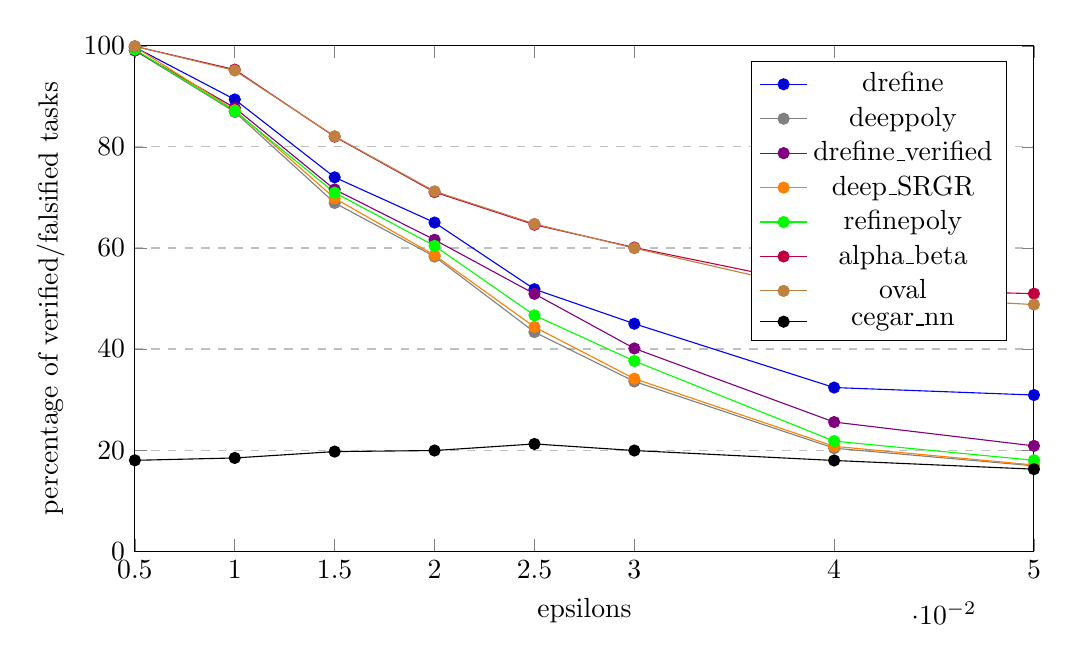
\begin{tikzpicture}
    \begin{axis}[
        xlabel={epsilons},
        ylabel={percentage of verified/falsified tasks},
        width=13cm,
        height=8cm,
        xmin=0.005, xmax=0.05,
        ymin=0, ymax=100,
        xtick={0.005,0.01,0.015,0.02,0.025,0.03,0.04,0.05},
        ytick={0,20,40,60,80,100},
        legend pos=north east,
        legend entries={drefine,deeppoly, drefine\_verified, deep\_SRGR, refinepoly, alpha\_beta, oval, cegar\_nn},
        ymajorgrids=true,
        grid style=dashed,
    ]
    \addplot+[
        color=blue,
        mark=*,
    ]
    coordinates {
        (0.005,99.72)(0.01,89.39)(0.015,73.98)(0.02,65.03)(0.025,51.84)(0.03,45.01)(0.04,32.38)(0.05,30.9)
    };

    \addplot[
        color=gray,
        mark=*,
    ]
    coordinates {
        (0.005,99.07)(0.01,86.9)(0.015,68.91)(0.02,58.3)(0.025,43.35)(0.03,33.58)(0.04,20.38)(0.05,16.89)
    };

    \addplot[
        color=violet,
        mark=*,
    ]
    coordinates {
        (0.005,99.07)(0.01,87.73)(0.015,71.58)(0.02,61.62)(0.025,50.92)(0.03,40.12)(0.04,25.55)(0.05,20.84)
    };

    \addplot[
        color=orange,
        mark=*,
    ]
    coordinates {
        (0.005,99.8)(0.01,87.26)(0.015,69.83)(0.02,58.57)(0.025,44.37)(0.03,34.13)(0.04,20.75)(0.05,17.06)
    };

    \addplot[
        color=green,
        mark=*,
    ]
    coordinates {
        (0.005,99.26)(0.01,87.08)(0.015,70.94)(0.02,60.42)(0.025,46.67)(0.03,37.63)(0.04,21.78)(0.05,17.99)
    };

    \addplot[
        color=purple,
        mark=*,
    ]
    coordinates {
        (0.005,99.9)(0.01,95.29)(0.015,82.02)(0.02,71.05)(0.025,64.60)(0.03,60.09)(0.04,51.98)(0.05,50.96)
    };

    \addplot[
        color=brown,
        mark=*,
    ]
    coordinates {
        (0.005,99.9)(0.01,95.11)(0.015,82.1)(0.02,71.21)(0.025,64.76)(0.03,59.96)(0.04,50.92)(0.05,48.8)
    };

    \addplot[
        color=black,
        mark=*,
    ]
    coordinates {
        (0.005,17.98)(0.01,18.45)(0.015,19.71)(0.02,19.92)(0.025,21.22)(0.03,19.92)(0.04,17.95)(0.05,16.23)
    };


    \end{axis}

\end{tikzpicture}
    \caption{Epsilon wise comparison with related techniques}
    \label{res:ep:milp_with_milp}
\end{figure}
\todo{recall what is epsilon... x axis label can perhaps be written out more}

\begin{table}[b]
  \footnotesize
    \centering
    \begin{tabular}{|c|c|c|c|c|c|c|c|c|}
        \hline
      - & \textbf{total} & \textbf{cegar\_} & \textbf{deeppoly} & \textbf{kPoly} & \textbf{deepSRGR} & $\alpha \beta-$ & \textbf{oval} & \textbf{drefine} \\
        &     & \textbf{\_nn}& & & & \textsc{CROWN}& & \\
        \hline
        \textbf{cegar\_nn} & 1638 & 0 & 713 & 609 & 687 & 217 & 238 & 417 \\ 
        \hline
        \textbf{deeppoly} & 4633 & 3708 & 0 & 0 & 0 & 63 & 66 & 0  \\ 
        \hline
        \textbf{kPoly} & 4789 & 3760 & 156 & 0 & 114 & 63 & 66 & 14  \\ 
        \hline
        \textbf{deepSRGR} & 4687 & 951 & 54 & 2 & 0 & 63 & 66 & 0 \\ 
        \hline
        \alphabeta{} & 6242 & 4821 & 1672 & 1516 & 1618 & 0 & 84 & 1095  \\
        \hline
        \textbf{Oval} & 6189 & 4789 & 1622 & 1466 & 1568 & 31 & 0 & 1052 \\
        \hline
        \textbf{drefine} & 5327 & 4106 & 694 & 552 & 640 & 180 & 190 & 0  \\
        \hline
    \end{tabular}
    \caption{Comparison of tools, example row \kpoly{} and column \deeppoly{} represents 156 benchmark instances on which \kpoly{} but \deeppoly{} fails}
    \label{tb:matrix}
\end{table}


%--------------------- DO NOT ERASE BELOW THIS LINE --------------------------

%%% Local Variables:
%%% mode: latex
%%% TeX-master: "../main"
%%% End:

